\documentclass[11pt,a4paper]{article}

\usepackage[utf8]{inputenc}
\usepackage[T1]{fontenc}
\usepackage[spanish,es-tabla]{babel}
\usepackage[margin=1.8cm]{geometry}
\usepackage{booktabs}
\usepackage{tabularx}
\usepackage{enumitem}
\usepackage{amsmath}
\usepackage{graphicx}
\usepackage[hidelinks]{hyperref}

\setlength{\parindent}{0pt}
\setlength{\parskip}{4pt}
\setlist[itemize]{nosep,leftmargin=1.4em,topsep=2pt}

\begin{document}

\begin{center}
    {\LARGE \textbf{FICHA T\'ECNICA EJECUTIVA --- TERRAPULSE AI}}\\[4pt]
    {\small Especificaci\'on de Arquitectura y Capacidades del Sistema Geoespacial y Geof\'isico}
\end{center}
\vspace{2pt}
\hrule
\vspace{6pt}

\section*{1. Datos Generales}
\begin{tabularx}{\textwidth}{@{}l X l X@{}}
\toprule
\textbf{Nombre del Proyecto} & TerraPulse AI & \textbf{Versi\'on} & 1.0 \\
\textbf{Tipo de Software} & \multicolumn{3}{l}{Plataforma Web de An\'alisis Geoespacial y Geof\'isico (SaaS Cient\'ifico)} \\
\textbf{Contexto Técnico} & \multicolumn{3}{l}{NASA Space Apps Challenge 2026 (\emph{Be an Earth System Trend Detective})} \\
\textbf{Licencia y Datos} & \multicolumn{3}{l}{C\'odigo reproducible con trazabilidad extrema sobre productos p\'ublicos NASA/ASF} \\
\addlinespace[2pt]
\textbf{P\'ublico Objetivo} & \multicolumn{3}{l}{Agencias de Protecci\'on Civil, investigadores ambientales y gestores de riesgo.} \\
\bottomrule
\end{tabularx}

\section*{2. Descripci\'on Corta}
TerraPulse AI es una plataforma anal\'itica geoespacial y geof\'isica de extremo a extremo que procesa observaciones de radar de apertura sint\'etica (SAR) en banda L de la misi\'on NASA--ISRO NISAR sin requerir la descarga de escenas completas ($\sim 7\text{ GB}$). Resuelve la inspecci\'on radiom\'etrica bajo demanda mediante lectura remota por bloques HTTPS (HDF5/h5py), la detecci\'on cuantitativa y auditable de cambios superficiales ($\Delta\gamma^0$) con control estricto de comparabilidad orbital/CRID, y la modelaci\'on f\'isica acoplada sobre Regiones de Inter\'es (ROI) arbitrarias (topograf\'ia 3D con factibilidad geom\'etrica SAR, propagaci\'on s\'ismica el\'astica e irradiancia solar).

\section*{3. Stack Tecnol\'ogico}
\begin{tabularx}{\textwidth}{@{}l X@{}}
\toprule
\textbf{Capa} & \textbf{Tecnolog\'ias, Motores y Librer\'ias} \\
\midrule
\textbf{Backend y Pipeline} & Python 3.11, Django 5.2 (GeoDjango), Django REST Framework (DRF 3.18), \texttt{h5py} (streaming HDF5 por ventanas HTTP), \texttt{rasterio}/GDAL (COG EPSG:3857/32615), \texttt{xarray}, \texttt{geopandas}, \texttt{shapely}, \texttt{pyproj}, \texttt{scipy}, \texttt{earthaccess} y \texttt{asf\_search}. \\
\addlinespace[3pt]
\textbf{Frontend (SPA)} & React 19, TypeScript 6, Vite 8, MapLibre GL JS 6 (renderizado vectorial/r\'aster WebGL 2D), Three.js 0.187 (bloques topogr\'aficos 3D con \texttt{React.lazy}) y Chart.js 4 (telemetr\'ia SAR, sismogramas a $50\text{ Hz}$ e histogramas). \\
\addlinespace[3pt]
\textbf{Base de Datos y Despliegue} & PostgreSQL 16 con extensi\'on espacial PostGIS 3.4 (\texttt{postgis/postgis:16-3.4}), contenedorizaci\'on mediante Docker y Docker Compose con persistencia en vol\'umenes y ejecuci\'on de subprocesos aislados por grupos de sesi\'on POSIX. \\
\bottomrule
\end{tabularx}

\section*{4. M\'odulos Principales (Capacidades)}

\noindent
\begin{minipage}[c]{0.60\textwidth}
    \textbf{4.1. Mapa de Cambio SAR (GCOV)}\\[2pt]
    Calcula la diferencia temporal $\Delta\gamma^0_{\text{dB}} = \gamma^0_{\text{dB},t_2} - \gamma^0_{\text{dB},t_1}$ (HH/HV) promediando potencia lineal antes de convertir a decibeles, con verificaci\'on estricta de identidad de malla, CRID y madurez.
    \begin{itemize}
        \item \textbf{Entradas:} Pol\'igono ROI (\texttt{EPSG:4326}), par de escenas NISAR \texttt{L2\_PR\_GCOV} (Freq A, banda L), factor \emph{multilook} ($2 \times 2$, $5 \times 5$, $10 \times 10$) y umbral de cambio ($\pm 1.5\text{ a }\pm 6.0\text{ dB}$).
        \item \textbf{Salidas:} R\'asteres GeoTIFF/COG (\texttt{delta\_dB.tif}, \texttt{zscore.tif}, \texttt{cambio.tif}), PNG web ($\pm 6\text{ dB}$), m\'etricas de \'area afectada ($\text{km}^2$ y \%), ruido robusto $\sigma_{\text{MAD}}$ y gr\'aficas Chart.js (histogramas $\gamma^0$, incidencia y QA).
    \end{itemize}
\end{minipage}%
\hfill
\begin{minipage}[c]{0.40\textwidth}
    \centering
    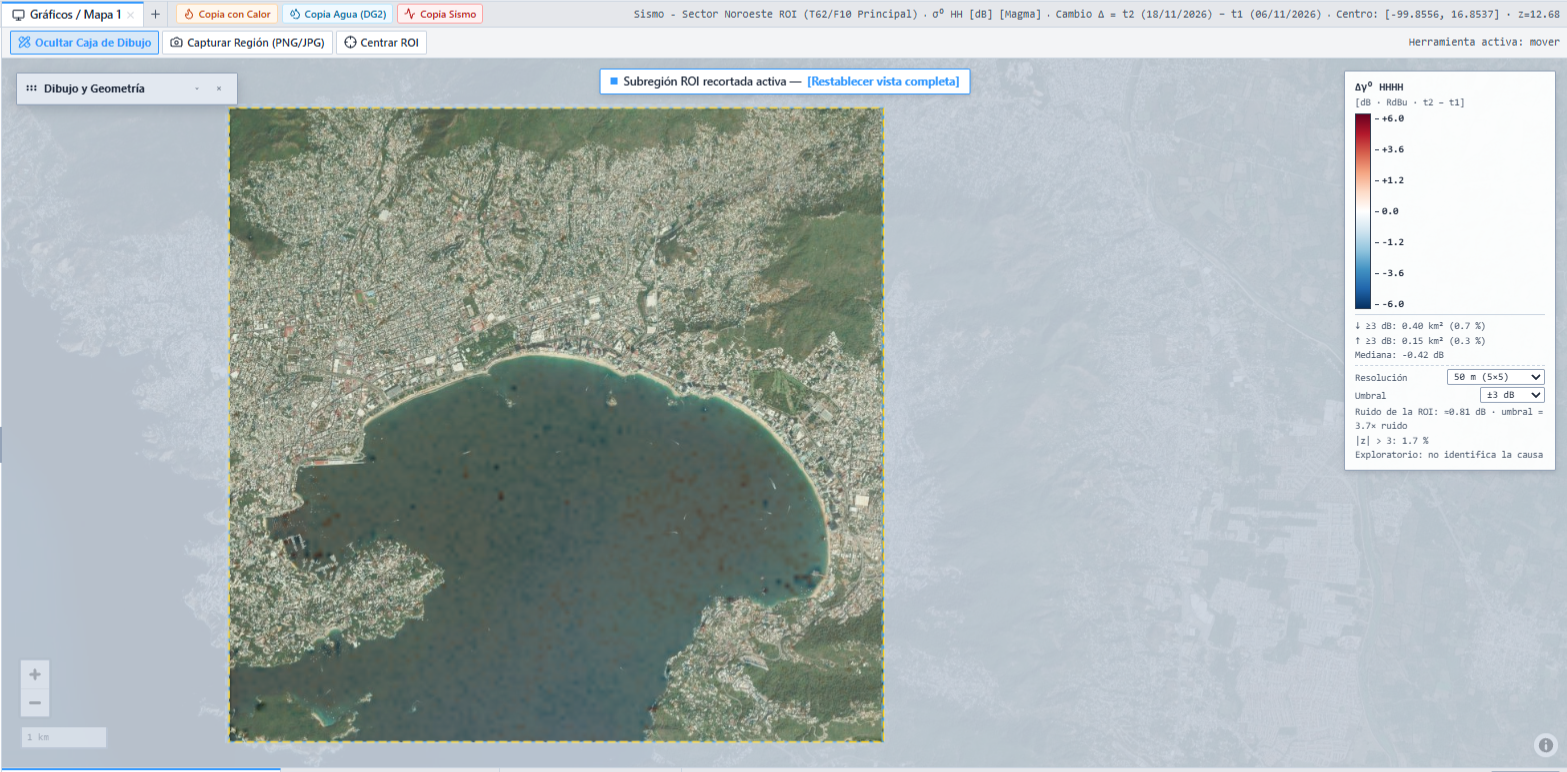
\includegraphics[width=0.95\linewidth]{fig/IMG_cambio_sar_mapa_delta.png}
\end{minipage}

\vspace{15pt}

\noindent
\begin{minipage}[c]{0.60\textwidth}
    \textbf{4.2. Visor 3D (M\'ascara SAR)}\\[2pt]
    Reconstruye una malla topogr\'afica de $161 \times 161$ v\'ertices en Three.js con filtro anti-picos $3 \times 3$ y eval\'ua la pendiente proyectada hacia el vector del haz lateral NISAR ($\theta_i \approx 43^\circ$) para diagnosticar distorsiones geom\'etricas.
    \begin{itemize}
        \item \textbf{Entradas:} Geometr\'ia ROI activa, teselas de elevaci\'on AWS Terrarium (decodificaci\'on nativa $1:1$ en metros), mosaico \'optico \emph{Esri World Imagery}, direcci\'on orbital (ASC T62/F10 o DESC T55/F80) y exageraci\'on vertical ($1.0\times\text{ a }5.0\times$).
        \item \textbf{Salidas:} Escena 3D interactiva WebGL (modos Satelital, Hipsom\'etrico, M\'ascara SAR y Wireframe), desglose porcentual de factibilidad (\emph{layover}, sombra radar, pendiente cr\'itica $> 15^\circ$ y suelo confiable), telemetr\'ia ($h_{\min}$, $h_{\max}$, $\Delta z$) y captura PNG.
    \end{itemize}
\end{minipage}%
\hfill
\begin{minipage}[c]{0.40\textwidth}
    \centering
    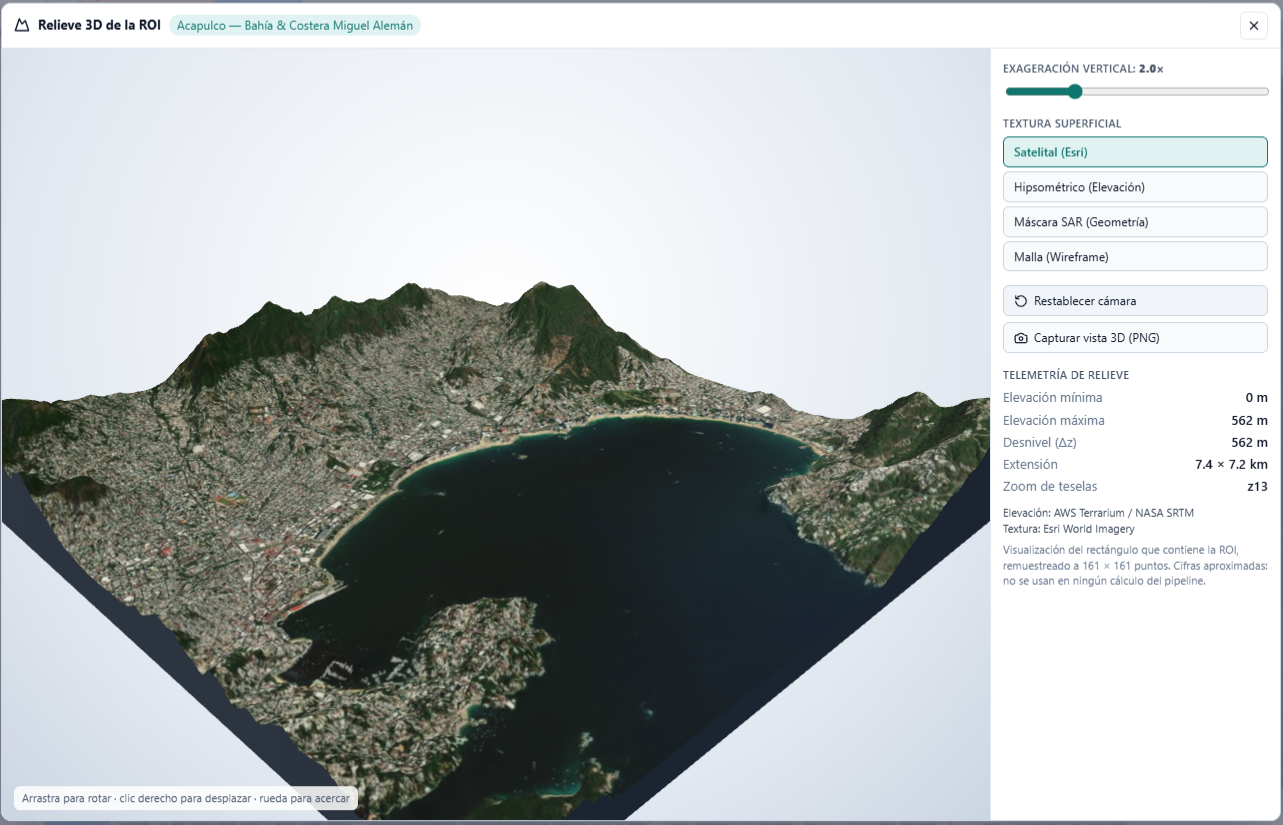
\includegraphics[width=0.95\linewidth]{fig/IMG_visor_3d_satelital.png}
\end{minipage}

\vspace{15pt}

\noindent
\begin{minipage}[c]{0.60\textwidth}
    \textbf{4.3. Simulador S\'ismico (GMPE, ondas P/S)}\\[2pt]
    Modela en tiempo real la atenuaci\'on s\'ismica regional para M\'exico (subducci\'on interplaca, intraplaca profundo y cortical) y la elastodin\'amica de ondas de cuerpo entre el hipocentro y una estaci\'on virtual.
    \begin{itemize}
        \item \textbf{Entradas:} Coordenadas epicentrales $(\lambda, \phi)$, magnitud de momento ($M_w$), profundidad focal ($h$), mecanismo de falla, velocidad de onda de corte superficial ($V_{s30}$) y posici\'on de la estaci\'on receptora.
        \item \textbf{Salidas:} Anillos geod\'esicos de isosisma en MapLibre GL, curva de atenuaci\'on PGA ($g$/Gal) e intensidad MMI continua, tiempos de arribo ($t_P$ a $6.0\text{ km/s}$, $t_S$ a $3.5\text{ km/s}$), ventana de alerta $\Delta t$, sismograma sint\'etico $a(t,D)$ a $50\text{ Hz}$ y espectrograma.
    \end{itemize}
\end{minipage}%
\hfill
\begin{minipage}[c]{0.40\textwidth}
    \centering
    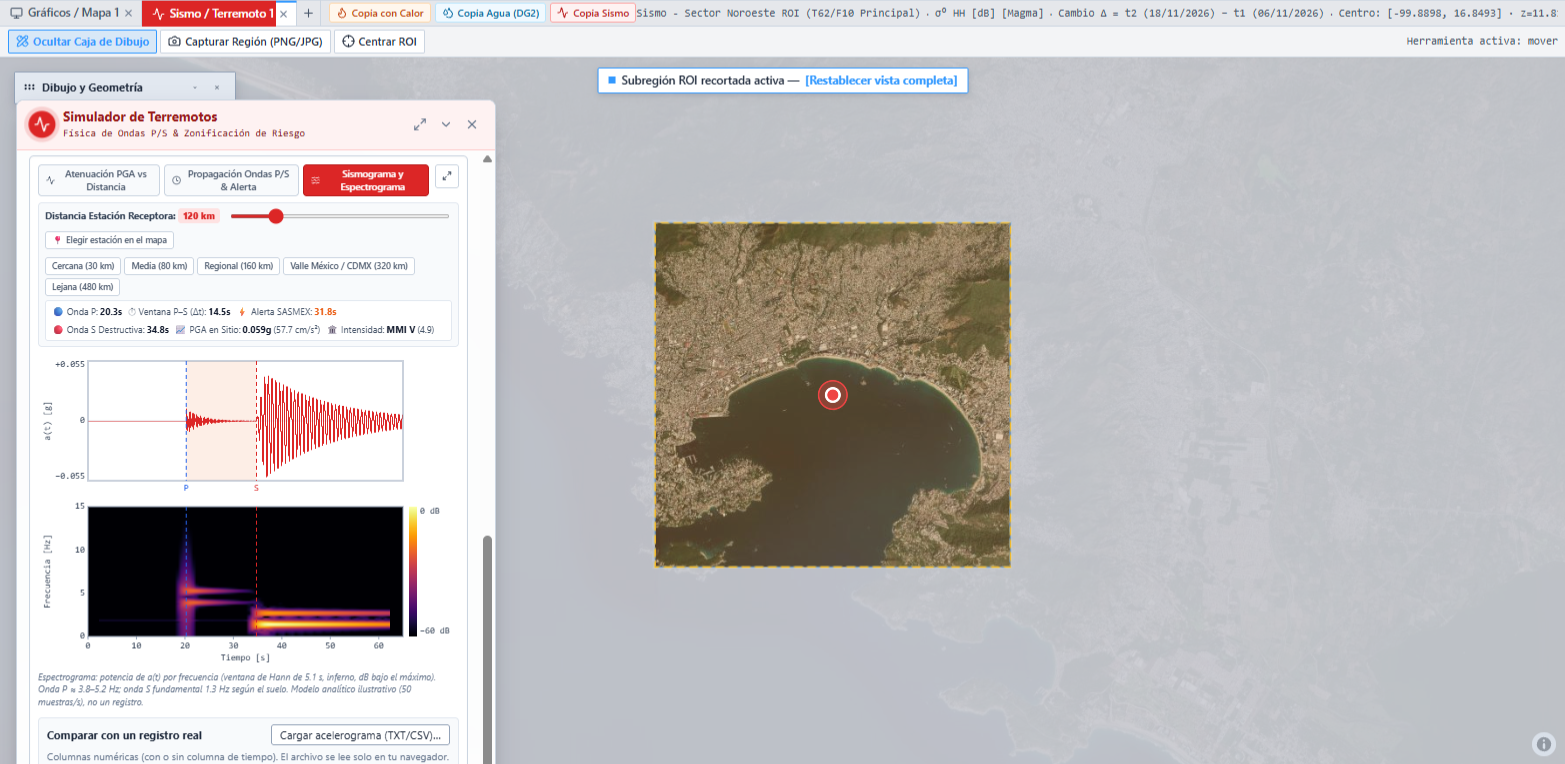
\includegraphics[width=0.95\linewidth]{fig/IMG_sismo_sismograma_espectrograma.png}
\end{minipage}

\vspace{15pt}

\noindent
\begin{minipage}[c]{0.60\textwidth}
    \textbf{4.4. Simulador Solar}\\[2pt]
    Calcula la irradiancia solar directa incidente sobre topograf\'ia real integrando efem\'erides astron\'omicas de alta precisi\'on (SPA), extinci\'on atmosf\'erica de cielo despejado y horizonte de auto-sombreado topogr\'afico.
    \begin{itemize}
        \item \textbf{Entradas:} Pol\'igono ROI (\texttt{EPSG:4326}), granulares \texttt{NASADEM\_HGT v001} ($1'' \approx 30\text{ m}$), fecha/hora local con zona IANA, factor de intensidad ($\%$), temperatura ambiente ($^\circ\text{C}$), presi\'on barom\'etrica (hPa) y turbidez de Linke.
        \item \textbf{Salidas:} GeoTIFF num\'erico de irradiancia incidente ($\text{W/m}^2$ en UTM), mapa de calor PNG (\texttt{EPSG:4326}, paleta \emph{inferno}), vectores solares (elevaci\'on aparente, azimut, DNI ajustado) y muestreo puntual interactivo (\texttt{/sample}).
    \end{itemize}
\end{minipage}%
\hfill
\begin{minipage}[c]{0.40\textwidth}
    \centering
    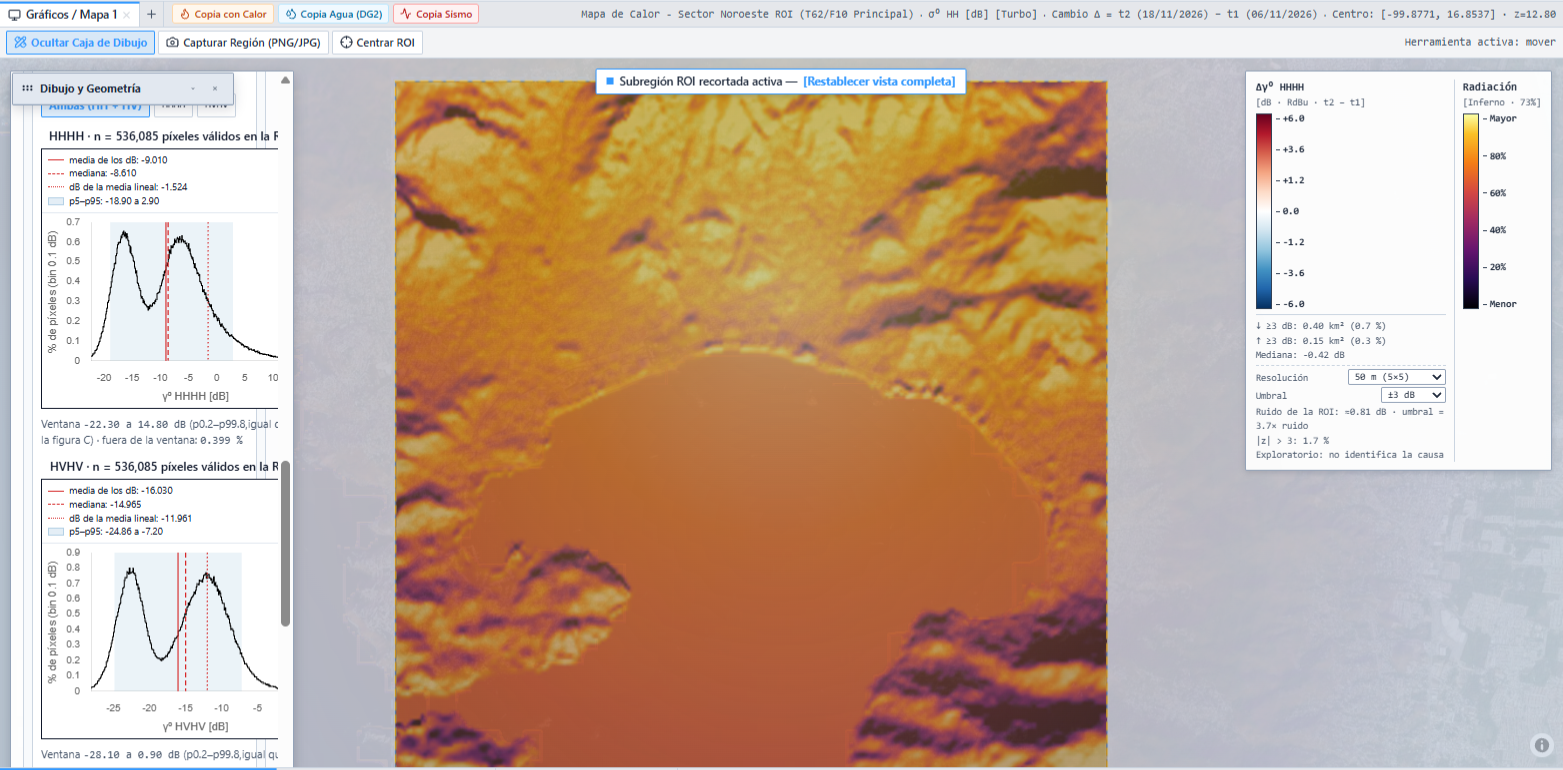
\includegraphics[width=0.95\linewidth]{fig/IMG_simulador_solar_heatmap_ui.png}
\end{minipage}

\vspace{15pt}

\noindent
\begin{minipage}[c]{0.60\textwidth}
    \textbf{4.5. Simulador de Lluvia y Encharcamientos}\\[2pt]
    Modela la acumulaci\'on superficial de agua y susceptibilidad hidr\'aulica (esquema DG2 2D / escorrent\'ia topogr\'afica) sobre la ROI a partir del modelo digital de elevaci\'on y escenarios sint\'eticos de precipitaci\'on.
    \begin{itemize}
        \item \textbf{Entradas:} Pol\'igono ROI y dominio (\texttt{EPSG:4326}), elevaci\'on \texttt{NASADEM\_HGT v001} reproyectada a malla m\'etrica UTM, l\'amina acumulada ($\text{mm}$), duraci\'on ($\text{s}$, $\text{min}$, $\text{h}$), perfil temporal (\texttt{uniform\_balanced}), rugosidad de Manning ($n$) y condiciones de frontera (\texttt{free}/\texttt{closed}).
        \item \textbf{Salidas:} R\'asteres COG de tirante/calado de agua ($\text{m}$ sobre el lecho local, \texttt{*.wd.tif}) y envolvente m\'axima, capa superpuesta en MapLibre GL, m\'etricas de celdas h\'umedas/\'area anegada e histogramas de severidad e intensidad media.
    \end{itemize}
\end{minipage}%
\hfill
\begin{minipage}[c]{0.40\textwidth}
    \centering
    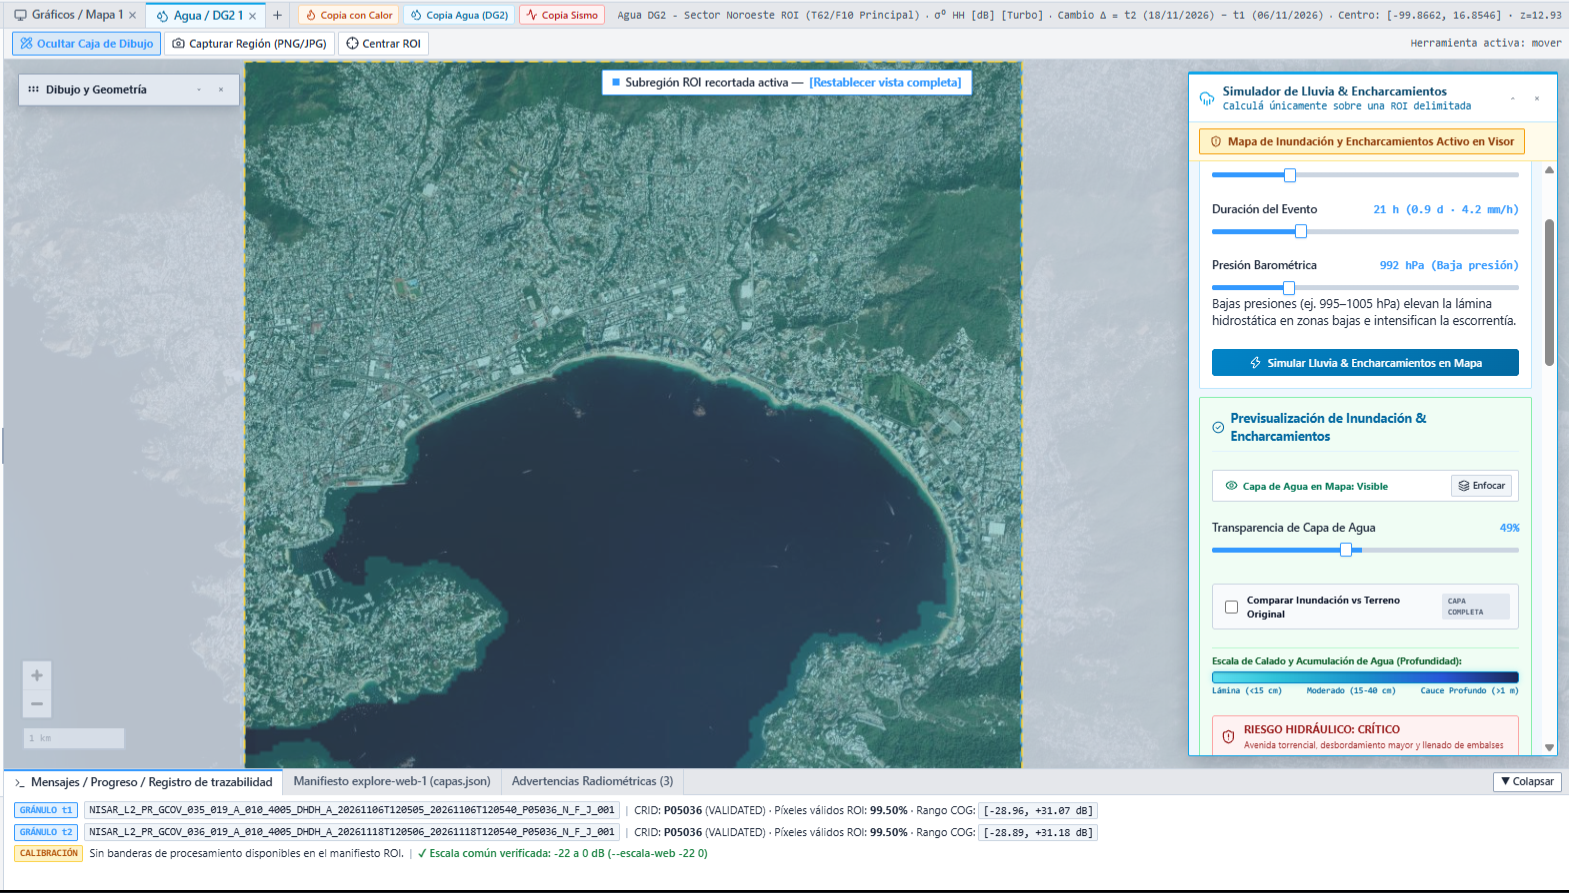
\includegraphics[width=0.95\linewidth]{fig/IMG_simulador_agua_encharcamientos.png}
\end{minipage}

\section*{5. Fuentes de Datos}
\begin{tabularx}{\textwidth}{@{}l l X@{}}
\toprule
\textbf{Fuente / Proveedor} & \textbf{Producto / Nivel} & \textbf{Uso Operativo en la Plataforma} \\
\midrule
\textbf{NASA Earthdata \& ASF} & Cat\'alogo CMR / Vertex & Autenticaci\'on OAuth/netrc, b\'usqueda espacial y lectura parcial por rangos HTTP de bloques HDF5 dentro de la ROI. \\
\addlinespace[2pt]
\textbf{NASA--ISRO NISAR} & \texttt{L2\_PR\_GCOV} (Freq A) & Covarianza geocodificada en banda L ($\lambda \approx 24\text{ cm}$), polarizaciones HH y HV, m\'ascara de subfranja y \'angulo de incidencia. \\
\addlinespace[2pt]
\textbf{NASA LP DAAC} & \texttt{NASADEM\_HGT v001} & Modelo digital de elevaci\'on cient\'ifico ($1'' \approx 30\text{ m}$, mallas HGT $3601 \times 3601$ de 16 bits) para simulaci\'on solar e hidr\'aulica. \\
\addlinespace[2pt]
\textbf{AWS Terrarium / Esri} & Teselas PNG $256 \times 256$ & Decodificaci\'on nativa $1:1$ en metros para el visor de relieve 3D en cliente y recubrimiento \'optico \emph{Esri World Imagery}. \\
\bottomrule
\end{tabularx}

\section*{6. Requisitos y Restricciones Operativas}
\begin{itemize}
    \item \textbf{Tama\~no M\'aximo y Geometr\'ia de ROI:} Pol\'igono GeoJSON cerrado en \texttt{EPSG:4326} (4 a 100 v\'ertices, sin agujeros) con caja envolvente restringida a un m\'aximo estricto de $0.6^\circ \times 0.6^\circ$ ($\approx 65\text{ km}$ por lado) para procesamiento SAR y hasta $3.0^\circ$ para el visor 3D en cliente.
    \item \textbf{Resoluci\'on Multilook Din\'amica y Umbrales:} Muestreo espacial configurable en tiempo real a $20\text{ m}$ ($2 \times 2$), $50\text{ m}$ ($5 \times 5$, por defecto) y $100\text{ m}$ ($10 \times 10$) desde los COG de potencia lineal precalculados ($\sim 0.1\text{--}1.5\text{ s}$ sin re-descargar de ASF), con umbrales de clasificaci\'on de $\pm 1.5\text{ a }\pm 6.0\text{ dB}$ y alerta autom\'atica de \emph{speckle} cuando $\text{umbral} < 3\sigma_{\text{MAD}}$.
    \item \textbf{Cach\'e Transaccional y Concurrencia:} Identificadores deterministas SHA-256 por geometr\'ia y versi\'on de c\'odigo (\texttt{roi-web-3}), directorios at\'omicos de bloqueo (\texttt{reservation/} y \texttt{<combo>.lock}), retenci\'on LRU de las 4 combinaciones $\Delta\gamma^0$ m\'as recientes, verificaci\'on de integridad de granulares NASADEM por recibo local SHA-256/CRC y l\'imite de 3 trabajos activos concurrentes (HTTP 429) con \emph{timeout} duro de 30 minutos.
    \item \textbf{Infraestructura de Despliegue (Hardware):} El entorno Dockerizado requiere un servidor o instancia Cloud (p.~ej., AWS EC2 / VPS Linux x86\_64) con un m\'inimo de $4\text{ vCPU}$, $8\text{ GB}$ de RAM ($16\text{ GB}$ recomendados para procesamiento matricial concurrente de bloques HDF5/COG) y $50\text{ GB}$ de almacenamiento SSD NVMe para vol\'umenes PostGIS y cach\'e transaccional de r\'asteres (\texttt{data/}).
\end{itemize}

\section*{7. Referencias}
{\small
\begin{itemize}
    \item \textbf{4.1. Mapa de Cambio SAR (GCOV) y Fuentes NISAR:}
    [1] NASA--ISRO SAR (NISAR) Mission \& Products Overview (\url{https://nisar.jpl.nasa.gov/} y \url{https://nisar-docs.asf.alaska.edu/products-overview/});
    [2] Alaska Satellite Facility (ASF) NISAR Documentation \& Data Availability (\url{https://nisar-docs.asf.alaska.edu/availability-overview/} y \url{https://search.asf.alaska.edu/});
    [3] ISCE3 Radar Processing Framework (\url{https://github.com/isce-framework/isce3}) y NASA Earthdata Search (\url{https://search.earthdata.nasa.gov/}).
    \item \textbf{4.2. Visor 3D (M\'ascara SAR) y Modelos Digitales de Elevaci\'on:}
    [1] Horn, B.~K.~P. (1981). Hill shading and the reflectance map. \emph{Proceedings of the IEEE}, 69(1), 14--47 (\texttt{doi:10.1109/PROC.1981.11918});
    [2] NASA LP DAAC (2025). \emph{NASADEM User Guide, Version 1.3} (colecci\'on \texttt{NASADEM\_HGT v001}, \url{https://lpdaac.usgs.gov/documents/2237/NASADEM_User_Guide_V13.pdf});
    [3] AWS Open Data Terrain Tiles (\emph{Terrarium Format Specification}, \url{https://s3.amazonaws.com/elevation-tiles-prod/terrarium/}) y \emph{Esri World Imagery}.
    \item \textbf{4.3. Simulador S\'ismico (GMPE, ondas P/S):}
    [1] Arroyo, D., Garc\'ia, D., Ordaz, M., Mora, M.~A. y Singh, S.~K. (2010). Strong ground-motion relations for Mexican interplate earthquakes. \emph{Journal of Seismology}, 14, 769--785 (\texttt{doi:10.1007/s10950-010-9200-0});
    [2] Garc\'ia, D., Singh, S.~K., Herr\'aiz, M., Ordaz, M. y Pacheco, J.~F. (2005). Inslab earthquakes of Central Mexico: peak ground-motion parameters and response spectra. \emph{Bulletin of the Seismological Society of America}, 95(6), 2272--2282 (\texttt{doi:10.1785/0120050072});
    [3] Wald, D.~J., Quitoriano, V., Heaton, T.~H. y Kanamori, H. (1999). Relationships between peak ground acceleration, peak ground velocity, and Modified Mercalli Intensity in California. \emph{Earthquake Spectra}, 15(3), 557--564;
    [4] Hanks, T.~C. y Kanamori, H. (1979). A moment magnitude scale. \emph{Journal of Geophysical Research}, 84(B5), 2348--2350.
    \item \textbf{4.4. Simulador Solar:}
    [1] Reda, I. y Andreas, A. (2004). Solar position algorithm for solar radiation applications. \emph{Solar Energy}, 76(5), 577--589 (\texttt{doi:10.1016/j.solener.2003.12.003});
    [2] Ineichen, P. y Perez, R. (2002). A new airmass independent formulation for the Linke turbidity coefficient. \emph{Solar Energy}, 73(3), 151--157 (\texttt{doi:10.1016/S0038-092X(02)00045-2});
    [3] Kasten, F. y Young, A.~T. (1989). Revised optical air mass tables and approximation formula. \emph{Applied Optics}, 28(22), 4735--4738 (\texttt{doi:10.1364/AO.28.004735});
    [4] Dubayah, R. y Rich, P.~M. (1995). Topographic solar radiation models for GIS. \emph{International Journal of Geographical Information Systems}, 9(4), 405--419 (\texttt{doi:10.1080/02693799508902046});
    [5] Holmgren, W.~F., Hansen, C.~W. y Mikofski, M.~A. (2018). pvlib python: a Python package for modeling solar energy systems. \emph{Journal of Open Source Software}, 3(29), 884 (\texttt{doi:10.21105/joss.00884}).
    \item \textbf{4.5. Simulador de Lluvia y Encharcamientos (Hidrodin\'amica DG2):}
    [1] Shaw, J., Kesserwani, G., Neal, J., Bates, P. y Sharifian, M.~K. (2021). LISFLOOD-FP 8.0: the new discontinuous Galerkin shallow-water solver for multi-core CPUs and GPUs. \emph{Geoscientific Model Development}, 14, 3577--3602 (\texttt{doi:10.5194/gmd-14-3577-2021});
    [2] Sharifian, M.~K., Kesserwani, G., Chowdhury, A.~A., Neal, J. y Bates, P. (2023). LISFLOOD-FP 8.1: new GPU accelerated solvers for faster fluvial/pluvial flood simulations. \emph{Geoscientific Model Development}, 16, 2391--2413 (\texttt{doi:10.5194/gmd-16-2391-2023});
    [3] University of Bristol Hydrology Research Group --- LISFLOOD-FP Documentation \& Zenodo Artifact (\url{https://www.bristol.ac.uk/geography/research/hydrology/models/lisflood/} y \url{https://zenodo.org/records/4073011}).
\end{itemize}
}

\end{document}
